% This file is part of Presto-HF, a matlab toolbox to identify a circuit from
% its response.
%
% SPDX-License-Identifier: AGPL-3.0-or-later
%
% Copyright 2025 by
%   Centre Inria de l'Université Côte d'Azur
%   2004, route des Lucioles
%   06902 Sophia Antipolis Cedex
%
% and by
%   Mines Paris - Armines
%   60, boulevard Saint-Michel
%   75006 Paris
%
% Contributors: Fabien Seyfert, Jean-Paul Marmorat, Martine Olivi
%
% Presto-HF is free software: you can redistribute it and/or modify it under
% the terms of the GNU Affero General Public License as published by the Free
% Software Foundation, either version 3 of the License, or (at your option) any
% later version.
%
% Presto-HF is distributed in the hope that it will be useful, but WITHOUT ANY
% WARRANTY; without even the implied warranty of MERCHANTABILITY or FITNESS FOR
% A PARTICULAR PURPOSE. See the GNU Affero General Public License for more
% details.
%
% You should have received a copy of the GNU Affero General Public License
% along with Presto-HF. If not, see <https://www.gnu.org/licenses/>.
%
\documentclass[12]{article}
\usepackage{epsfig,amsfonts,latexsym}
\usepackage{theorem}
\usepackage{graphicx}
\usepackage{amsmath}
\usepackage[frenchb]{babel}
\usepackage{xspace} 
% This file is part of Presto-HF, a matlab toolbox to identify a circuit from
% its response.
%
% SPDX-License-Identifier: AGPL-3.0-or-later
%
% Copyright 2025 by
%   Centre Inria de l'Université Côte d'Azur
%   2004, route des Lucioles
%   06902 Sophia Antipolis Cedex
%
% and by
%   Mines Paris - Armines
%   60, boulevard Saint-Michel
%   75006 Paris
%
% Contributors: Fabien Seyfert, Jean-Paul Marmorat, Martine Olivi
%
% Presto-HF is free software: you can redistribute it and/or modify it under
% the terms of the GNU Affero General Public License as published by the Free
% Software Foundation, either version 3 of the License, or (at your option) any
% later version.
%
% Presto-HF is distributed in the hope that it will be useful, but WITHOUT ANY
% WARRANTY; without even the implied warranty of MERCHANTABILITY or FITNESS FOR
% A PARTICULAR PURPOSE. See the GNU Affero General Public License for more
% details.
%
% You should have received a copy of the GNU Affero General Public License
% along with Presto-HF. If not, see <https://www.gnu.org/licenses/>.
%
\usepackage{ifthen}
\usepackage{amsmath}
\usepackage{amsfonts}
\newcommand{\fitem}{\protect\item}
\newcommand\testempty[3]{\def\xtoto{#1}\ifx\xtoto\empty #2\else#3\fi}
\newcommand{\entrieslabel}[1]{\texttt{#1}:\vspace{0.5em} \hfill}
\newenvironment{entry}[0]
{\begin{list}{}%
    { \renewcommand{\makelabel}{\entrieslabel}%
      \setlength{\labelwidth}{4em}%
      \setlength{\labelsep}{0.3em}%
      \setlength{\parsep}{0em}%
      \setlength{\itemsep}{0em}%
      \setlength{\leftmargin}{4.5em}%
      \setlength{\topsep}{0em}%
    }%
}%
{\end{list}}
\newcommand{\FuncDef}[5]{
{\bf Signature }\texttt{#1} \\
{\bf Sortie(s)}
\testempty{#2}{ aucune \\}{
\begin{entry}
#2
\end{entry}
}
{\bf Entr\'ee(s)}
\testempty{#3}{ aucune \\}{
\begin{entry}
#3
\end{entry}
}
{\bf Constante(s)}
\testempty{#4}{ aucune \\}{
\begin{entry}
#4
\end{entry}
}
{\bf Description}
\testempty{#5}{ none \\}{\\#5\\}
}





\def\prest{Presto-HF\xspace}
\newcommand{\HH}{H^2}
\newcommand{\HHb}{\overline{H}^2_0}

\def\CC{{\mathbb C}}
\def\DD{{\mathbb D}}
\def\NN{{\mathbb N}}
\def\ZZ{{\mathbb Z}}
\def\QQ{{\mathbb Q}}
\def\RR{{\mathbb R}}
\def\TT{{\mathbb T}}
\def\cW{{\cal W}}
\def\cS{{\cal S}}

\begin{document}
\title{Manuel pour l'utilisateur du logiciel \prest}
\author{Fabien Seyfert}
\maketitle


\tableofcontents
\newpage

\section{Introduction}

Le document suivant constitue le manuel utilisateur de la boite \`a
outils matlab \prest. Cette derni\`ere d\'evelopp\'ees \`a l'Inria
Sophia-Antipolis au sein du projet Miaou \`a pour but de fournir un
ensemble de m\'ethodes pour l'extraction d'un mod\`ele rationnel stable de
taille $2 \times 2$ \` a partir de donn\'ees fr\'equentielles ponctuelles
relatives \`a la matrice de r\'epartition d'un filtre
passe-bande hyperfr\'equence. Cette boite \`a outil utilise le moteur
d'approximation rationnelle RARL2. Enfin pour extraire une matrice de
couplage \`a partir d'un mod\`ele rationnel on pourra utiliser RGC.

Le document suivant est structur\'e en trois parties. Dans un premier
temps nous exposerons la d\'emarche math\'ematique et algorithmique que
nous avons choisie d'impl\'ementer au sein de \prest. Ensuite nous
d\'ecrirons pas \`a pas  le traitement d'un exemple sur la base de donn\'ees
d'un filtre dix p\^oles. Enfin nous terminerons en d\'etaillant les
arguments d'entr\'ee-sortie des principales fonctions de \prest.        

\section{Algorithmique g\'en\'erale}

Au niveau conceptuel la strat\'egie d'identification se d\'ecompose en
trois \'etapes qui sont:
\begin{itemize}

\item Identification et compensation des composantes de retard
\item D\'etermination d'un mod\`ele stable d'ordre \'elev\'e par
  compl\'etion analytique des donn\'ees 
\item D\'etermination d'un mod\`ele rationnel stable de degr\'e de MacMillan
  prescrit.
\end{itemize}

Dans ce qui suit nous noterons par $(w_i)$ les points de fr\'equence
normalis\'es correspondant aux mesures. Ceux-ci sont obtenus
classiquement par la transformation passe-bas qui envoie la bande
passante du filtre sur l'intervalle de fr\'equences normalis\'ees
$[-1,1]$. Les mesures concernant la matrice de r\'epartition du filtre
au point $w_i$ seront not\'ees
$$
S(w_i)=\left[
\begin{array}{cc}
S_{1,1}(w_i) & S_{1,2}(w_i) \\
S_{2,1}(w_i) & S_{2,2}(w_i) \\
\end{array}
\right].
$$

\subsection{D\'etermination des composantes de retard}
\label{sec:detret}
Nous supposons qu'un \og bon \fg mod\`ele pour nos donn\'ees mesur\'ees
est donn\'e par: 

\begin{equation}
\label{model:donnees}
H(w)=\frac{1}{q(jw)} \left[
\begin{array}{cc}
e^{j(w\alpha_{1,1}+\beta_{1,1})} p_{1,1}(jw) &
e^{j(w(\frac{\alpha_{1,1}+\alpha_{2,2}}{2})+\beta_{2,1})} p_{1,2}(jw) \\
e^{j(w(\frac{\alpha_{1,1}+\alpha_{2,2}}{2})+\beta_{2,1})} p_{2,1}(jw)& 
e^{j(w\alpha_{2,2}+\beta_{2,2})} p_{2,2}(jw) 
\end{array}
\right]
\end{equation}
o\`u $(p_{i,j},q)$ sont des polyn\^omes de la
variable $w$, les valeurs $(\alpha_{i,i})$ sont les composantes de retard
induites par les acc\`es et les valeurs $(\beta_{i,j})$ mod\'elisent des shifts
en fr\'equence possiblement induits par les instruments de mesure. Afin
de pouvoir nous ramener \`a un probl\`eme d'identification rationnelle
il nous faut d'abord identifier les composantes $(\alpha_{i,i})$ et
$(\beta_{i,j})$.  Nous
consid\'ererons dans un premier temps l'identification des composantes
de retard $(\alpha_{i,i})$.

Soit $I$ un sous-ensemble des fr\'equences 
de mesure d\'efini en fonction du param\`etre $w_c$ de la mani\`ere
suivante:
\begin{equation}
\label{wc:def}
I=\{w_i,\,\,|w_i| \geq w_c \}.
\end{equation}
On choisira $w_c$ de mani\`ere \`a ce que le module de $S_{1,1}$ et
$S_{2,2}$ se comporte de mani\`ere \og r\'eguli\`ere \fg sur $I$, i.e cela
n\'ecessite implicitement la pratique de mesures sur une 
bande plus large que la seule bande passante du filtre. Pour les
fr\'equences de $I$ nous ferons l'hypoth\`ese forte que les composantes
rationnelles de (\ref{model:donnees}) sont bien approch\'ees par les premiers
$n_c$ termes de leur d\'eveloppement de Taylor \`a l'infini (i.e
d\'eveloppement en $\frac{1}{w}$). Notons ici que la fonction $e^{j\alpha 
  w}$ n'admet pas de d\'eveloppement de Taylor \`a l'infini. Nous
d\'efinissons ( ici par exemple pour la voie $(1,1)$) le
probl\`eme d'optimisation dont la fonction co\^ut est la suivante:
 
\begin{equation}
\label{optim:ret}
\psi(\alpha)=\min_{(a_0,a_1 \dots a_{n_c-1}) \CC^{n_c-1}}
\sum_{w_i \in I} \left | 
\sum_{k=0}^{n_c} \frac{a_k}{w_i^k} - S_{1,1}(w_i)e^{-j \alpha w_i}
\right |^2  
\end{equation}

La compensation optimale sera alors d\'efinie comme
la valeur $\alpha_{0}$ de $\alpha$ pour laquelle $\psi$ atteint son minimum sur
$\RR$.
L'id\'ee intuitive  derri\`ere cette
mani\`ere de faire consiste \`a exploiter le fait que pour des
fr\'equences assez lointaines de la bande passante le mod\`ele
rationnel du filtre se comporte comme un polyn\^ome en $\frac{1}{w}$ de bas
degr\'e: la composante de retard perturbe cette propri\'et\'e et permet
ainsi son identification. Si l'analyse th\'eorique de cette
m\'ethodologie est encore en cours (pour essayer de quantifier sa
pr\'ecision dans le pire des cas), les exp\'eriences men\'ees sur des
donn\'ees th\'eoriques et mesur\'ees plaident tr\`es largement en sa
faveur; les valeurs $n_c=3$ et $w_c=2.5$ donnent de bons r\'esultats
sur l'ensemble des exemples fournit par Alcatel. 

On proc\`ede de m\^eme sur la voie $(2,2)$, ce qui permet donc d'avoir
des estim\'ees pour tous les $(\alpha_{i,i})$ du mod\`ele
(\ref{model:donnees}). La d\'etermination des $\beta_{i,j}$ se fera
apr\`es l'\'etape de compl\'etion analytique qui suit.     


\subsection{Compl\'etion analytique}
\label{sec:comp}
A bien y regarder la m\'ethode pr\'ec\'edente fournit pour les voies
$(1,1)$ et $(2,2)$ un comportement estim\'e (sous forme de deux polyn\^omes
en $\frac{1}{w}$) de ces derni\`eres pour les fr\'equences en dehors de
la bande de mesure. Mais comment s'assurer que ce comportement est bien
conforme au caract\`ere stable et dissipatif du filtre \'etudi\'e ? Un
l\'eger perfectionnement du probl\`eme d'optimisation associ\'e au terme de droite 
de (\ref{optim:ret}) permet, comme nous allons le voir, de r\'epondre \`a
la question. 


Dans le cas d'une fraction rationnelle la stabilit\'e est
caract\'eris\'ee par l'appartenance des p\^oles de cette derni\`ere au
demi-plan gauche ouvert. Ceci est \'equivalent au caract\`ere analytique de cette fonction 
dans le demi-plan droit. Maintenant, afin d'assurer la convexit\'e du
probl\`eme de compl\'etion que nous allons poser, nous consid\'ererons un ensemble de 
fonctions analytiques plus g\'en\'eral que les seuls fonctions
rationnelles stables. Il s'agit de l'espace de Hilbert $H^2$ form\'e des
fonctions $h$ analytiques dans le demi-plan droit (ouvert) et dont l'int\'egrale
suivante reste born\'ee sur toutes les droites verticales du demi-plan droit, i.e
\begin{equation}
\label{h2:def}
\forall \sigma>0,\,\,\int_{-\infty}^{+\infty}
\frac{|h(\sigma+iw)|^2}{1+w^2}dw < \infty.
\end{equation}
Une propri\'et\'e importante des fonctions de $H^2$ est que ces
derni\`eres admettent une extension ($L^2$ int\'egrable) \`a 
l'axe imaginaire. En ce sens $H^2$ appara\^it comme un sous-espace de
l'espace de Hilbert $L^2$ des fonctions complexes d\'efinies sur l'axe imaginaire
dont la norme d\'erive du produit scalaire suivant:
$$
<u,v>=\int_{-\infty}^{+\infty} \frac{u(iw) \bar{v(iw)}}{1+w^2}dw.
$$   
Le suppl\'ementaire orthogonal de $H^2$ dans $L^2$ est not\'e $\HHb$ et on a donc:
\begin{equation}
\label{L2:dirsum}
 L^2=H^2 \oplus  \HHb. 
\end{equation} 
Plus concr\`etement l'\'equation (\ref{L2:dirsum}) est souvent
interpr\'et\'ee comme le fait que toute fonction $L^2$ int\'egrable sur
l'axe imaginaire se d\'ecompose (orthogonalement) comme la somme d'une
fonction stable dans $H^2$ et d'une fonction instable dans $\HHb$.
On notera $P_{H^2}$ et $P_{\HHb}$ les projections orthogonales de
$L^2$ sur $H^2$ (resp. sur $\HHb$).

La variable $S$ d\'esigne maintenant nos donn\'ees dont les
composantes de retard ont \'et\'e compens\'ees par l'\'etape
pr\'ec\'edente. Nous supposerons que sur l'intervalle de mesure 
$$J=[min(w_i),max(w_i)]$$
chacune des composantes de $S$ d\'efinie une
fonction continue dont la valeur entre deux points de mesure est
d\'efinie par interpolation (par des splines par exemple). 
On d\'efinit alors un probl\`eme de compl\'etion polynomiale sous la forme du
programme d'optimisation suivant (ici pour $S_{1,1}$):
\begin{gather}
\min_p \sum_{w_i \in I} |S_{1,1}(w_i)-p(\frac{1}{w_i})|^2 \\
\begin{cases}
\nonumber
p \in \CC^{n_c}[X] \\
||P_{\HHb}(S_{1,1} \wedge p)||^2 \leq E_c \\
\forall w \in J_c,\,\,|p(\frac{1}{w})|^2 \leq 1.
\end{cases} 
\end{gather}
Dans ce qui pr\'ec\`ede $\CC^{n_c}[X]$ d\'esigne l'ensemble des
polyn\^omes \`a coefficients complexes de degr\'e au plus $n_c$, $J_c$
d\'esigne le compl\'ementaire de l'intervalle de mesure $J$, la notation 
$S_{1,1} \wedge p$ d\'esigne la fonction d\'efinie sur $J$ par $S_{1,1}(w)$
et sur $J_c$ par $p(\frac{1}{w})$, la double
barre $||.||$ d\'esigne la norme $L^2$ et $E_c$ est un param\`etre du
probl\`eme d'optimisation qui prend ses valeurs dans $\RR^+$. A haute
voix le programme (\ref{compl:optim1}) s'\'enonce comme suit: trouver
la compl\'etion polynomiale qui rende le mieux compte
de nos donn\'ees sur $I$ tout en satisfaisant aux contraintes
suivantes:
\begin{itemize}
\item les donn\'ees compl\'ement\'ees par $p$ ont une partie
  instable inf\'erieure \`a $E_c$ 
\item le module de la compl\'etion reste inf\'erieur \`a 1 sur $J_c$.
\end{itemize}
Le programme d'optimisation (\ref{compl:optim1}) prend tout son sens
lorsque l'ensemble admissible associ\'e est non-vide, c'est pourquoi
\prest r\'esout dans un premier temps le programme suivant:
\begin{gather}
\label{compl:optim2}
\min_p ||P_{\HHb}(S_{1,1} \wedge p)||^2 \\
\begin{cases}
\nonumber
p \in \CC^{n_c}[X] \\
\forall w \in J_c,\,\,|p(\frac{1}{w})|^2 \leq 1.
\end{cases} 
\end{gather}
dont l'ensemble admissible n'est pas vide (il contient 0). Si la valeur
optimale $E_{m}$ de (\ref{compl:optim2}) est inf\'erieure \`a $E_c$ alors
le programme (\ref{compl:optim1}) sera r\'esolu (son ensemble
admissible est alors non-vide), dans le cas contraire la solution de
(\ref{compl:optim2}) est renvoy\'ee. 

Comme nous le verrons plus tard dans la description d\'etaill\'ee des
proc\'edures de \prest la valeur de $E_c$ est donn\'ee sous la forme d'un
pourcentage de la norme $L^2$ des donn\'ees sur $J$. De m\^eme la
contrainte de $1$ pour le module pourra \^etre remplac\'ee par une valeur
calcul\'ee \`a partir des valeurs du module des donn\'ees en bord de
bande de mesure. Ceci est particuli\`erement vrais pour la compl\'etion
des \'el\'ements diagonaux $S_{1,2}$ et $S_{2,1}$ dont le module est
suppos\'e chuter en dehors de la bande de mesure. De plus, pour ces
\'el\'ements un certain nombre de z\'eros \`a l'infini (qui correspondent
\`a des z\'eros de $p$ en z\'ero) pourra \^etre prescrit \`a l'avance par l'utilisateur.

Nous noterons $m_{i,j}$ les quatre polyn\^omes obtenus gr\^ace \`a
l'\'etape de compl\'etion que nous venons de d\'ecrire.


\subsection{D\'etermination des shifts en fr\'equence}
\label{sec:shift}
Nous disposons maintenant d'une compl\'etion \og r\'ealiste \fg de nos
donn\'ees pour des fr\'equences en dehors de la bande de mesure $J$. Le
mod\`ele \'electrique du filtre sp\'ecifie que la matrice $S$ de ce
dernier doit \^etre \'egale \`a l'identit\'e \`a l'infinie. Il est donc
raisonnable d'identifier 
$$ \beta_{1,1}=\arg(m_{1,1}(0)) \mbox{  et  }
\beta_{2,2}=\arg(m_{2,2}(0)).$$
Pour simplifier les notations notons \`a nouveau $S$ les donn\'ees o\`u
les voies (1,1) et (2,2) ont \'et\'e compens\'ees (i.e multipli\'ees
par $e^{-i\beta_{1,1}}$ et $e^{-i\beta_{2,2}}$) gr\^ace \`a la remarque 
pr\'ec\'edente. 

La matrice de r\'epartition $G$ d'un filtre id\'eal est suppos\'ee \^etre
conservative, ce qui s'exprime math\'ematiquement par:
\begin{equation}
\label{orth:S}
 \overline G^tG=Id.
\end{equation}
Si l'on explicite composantes par composantes l'\'equation (\ref{orth:S}) on
obtient $|G_{1,1}|^2=1$, $|G_{2,2}|^2=1$ et l'\'equation d'orthogonalit\'e
suivante:
\begin{equation}
\label{orthrel:S}
\forall w \in \RR,\,\,G_{1,1}(iw)\overline {G_{1,2}(iw)} + G_{2,2}(iw)\overline
{G_{1,2}(iw)}
\end{equation}
en rappelant que $G_{1,2}=G_{2,1}$. La compensation $\beta_{2,1}$ sera
d\'etermin\'ee pour respecter au mieux la relation
d'orthogonalit\'e (\ref{orthrel:S}) sur l'ensemble des points de mesure. Une analyse simple montre qu'un tel $\beta_{2,1}$
n'est d\'efini qu'\`a $\pi$ pr\`es: \prest fera donc ici un choix arbitraire 
(ce dernier est d\'eterministe et gouvern\'e par un un param\`etre, voir 
section \ref{sec:det}). Cela est cependant moins grave qu'il n'y parait
puisqu'on montre que ce
choix n'influe au final que sur le signe de certains couplages qui lui est d\'etermin\'e par des consid\'erations
technologiques relatives aux vis et iris du filtre.

\subsection{D\'etermination d'un mod\`ele rationnel stable de degr\'e de
  MacMillan donn\'e}

On note \`a nouveau $S$ les donn\'ees cette fois compens\'ees par
l'ensemble des proc\'edures pr\'ec\'edemment d\'ecrites et $m_{i,j}$ les
polyn\^omes qui d\'eterminent les compl\'etions associ\'ees. 
On d\'efinit voie par voie,
$$
F_{i,j}=P_{\HH}(S_{i,j} \wedge m_{i,j}).$$
Les fonctions $F_{i,j}$ peuvent \^etre vues comme les repr\'esentants
stables de nos donn\'ees initiales. C'est \`a partir de ces fonctions
que nous allons d\'eterminer un mod\`ele rationnel stable de degr\'e de
MacMillan fix\'e de nos donn\'ees. Pour simplifier on pourra consid\'erer ici que le
degr\'e de MacMillan de la matrice de r\'epartition associ\'ee \`a un
filtre se confond avec ce qu'on appelle classiquement son ordre, i.e la
taille de la matrice de couplage de sa mod\'elisation \'electrique. Le logiciel RARL2 s'attaque au probl\`eme suivant,
\begin{gather}
\label{RARL2:optim}
\min_R |||F-R|||^2=\sum_{i,j} ||F_{i,j}-R_{i,j}||^2 \\
\begin{cases}
\nonumber
R \mbox{ rationnelle de taille }(2 \times 2) \\
Deg(R) \leq n_f \\
R \mbox{ stable }
\end{cases} 
\end{gather}   
o\`u $n_f$ est le degr\'e de MacMillan cible et constitue un param\`etre 
d'entr\'ee du logiciel. Sans rentrer dans les d\'etails de l'algorithme
qui sous-tend RARL2 on pourra retenir:
\begin{itemize}
\item la param\'etrisation des matrices rationnelles stables qu'utilise
  l'algorithme repose sur le calcul de param\`etres de Schur
\item afin de garantir la stabilit\'e de l'approximant calcul\'e il est
  essentiel que $F_{i,j} \in \HH$.
\end{itemize} 
Cette derni\`ere remarque explique notre \og acharnement \fg \`a obtenir un
mod\`ele de nos donn\'ees dans $H^2$ avant de passer \`a l'approximation 
rationnelle proprement dite. 

La boite \`a outils \prest fait appel \`a RARL2 pour l'\'etape
d'approximation rationnelle.  

\section{Un exemple pas \`a pas}


Nous traiterons ici l'exemple du calcul d'un mod\`ele rationnel \`a partir 
des mesures d'un filtre dix p\^oles fournit par Alcatel. 
\subsection{Initialisation}

Afin de pouvoir appeler les proc\'edures de \prest l'utilisateur doit
indiquer \`a matlab o\`u trouver ces derni\`eres. Il est conseill\'e de
faire cela en appelant la proc\'edure \verb+PrestoInit+ situ\'ee dans le
r\'epertoire \verb+presto+. Pour ce faire on pourra par exemple se placer
sous matlab dans ce r\'epertoire (utiliser cd) et taper
\begin{verbatim}
>> PrestoInit
\end{verbatim}
 
\subsection{Une structure pour les donn\'ees}
\label{sec:donnees}
Le point
d'entr\'ee de \prest est constitu\'e par une structure \'el\'ementaire 
\`a l'image de la variable \verb+Spb+ d\'ecrite par ce qui suit,
\begin{verbatim}
Spb = 

    value: [2x2x801 double]
     freq: [1x801 double]
     name: 'alc200601'
\end{verbatim}
Le champ \verb+value+ de \verb+Spb+ contient les mesure de la matrice
de r\'epartition sous la forme d'un tableau de dimension $2 \times 2
\times nd$ o\`u $nd$ est le nombre de point de mesures. Dans notre
exemple $nd=801$. Le champ \verb+freq+ est un vecteur
ligne sp\'ecifiant les fr\'equences {\bf normalis\'ees passe-bas}
des diff\'erentes mesures. Enfin, le champ \verb+name+ sp\'ecifie le nom que
l'utilisateur veut attribuer \`a son jeu de donn\'ees. Ce champ est
optionnel au sens o\`u il n'est requis de mani\`ere obligatoire par aucune 
des fonctions. \prest ne poss\`ede pour l'instant qu'un
parseur \'el\'ementaire (appelable par \verb+ParseS+) pour charger des
donn\'ees \`a partir d'un fichier ascii; il est donc recommand\'e
\`a chaque utilisateur d'\'ecrire un parseur pour son format
ascii favori. 

Pour des raisons de commodit\'e beaucoup des param\`etres relatifs aux
proc\'edures de \prest ont une valeur par d\'efaut, dont nous pensons
qu'elle \og fera l'affaire \fg dans la plus-part des cas. L'utilisateur peut
cependant sp\'ecifier la valeur de son choix pour ces param\`etres en
ajoutant un champ \verb+params+ \`a sa structure de d\'epart comme c'est 
le cas pour la structure \verb+Spb1+ ci dessous:
\begin{verbatim}
Spb1 = 

      freq: [401x1 double]
     value: [2x2x401 double]
    params: @GetMyDefaultValue
\end{verbatim}
Le champ \verb+params+ est un pointeur de fonction (voir manuel matlab,
function handle) 
qui indique ici le chemin d'appel d'une proc\'edure qui red\'efinit tout 
ou partie des param\`etres de \prest. A titre d'exemple le code de la
proc\'edure \verb+GetMyDefaultValue+ est ici le suivant,
\begin{verbatim}
function DVC=GetMyDefaultValue()

%     ************  Completion and delay determination  *******

DVC.CDAFS.delay_range=[-0.3:.001:0.3];
DVC.CDAFS.poly_order=4;
DVC.CDAFS.omega_lim=3.3;
DVC.CDAFS.causal_bound(1,1)=0.7;
DVC.CDAFS.causal_bound(2,2)=0.9;
DVC.CDAFS.modulus_factor(1,1)=1.01;
DVC.CDAFS.modulus_factor(2,2)=1.01;

\end{verbatim}
La proc\'edure \verb+GetMyDefaultValue+ renvoie une structure dont
chaque champ correspond \`a un param\`etre que l'utilisateur d\'esire
sp\'ecifier. Ici par exemple l'utilisateur d\'esire que l'ordre des
polyn\^omes utilis\'es lors de la d\'etermination du retard et de l'\'etape
de compl\'etion soit de 4. La description de l'ensemble des param\`etres
ainsi que de leurs syntaxes sera faite \`a la section \ref{sec:det}.

\subsection{Affichage des donn\'ees}

La proc\'edure \verb+Plot+ permet d'avoir acc\`es au diagramme de Nyquist de
la structure \verb+Spb+ en tapant,

\begin{verbatim}
>> PlotS(Spb)
\end{verbatim}

Matlab renvoie alors une fen\^etre graphique constitu\'ee du diagramme de
Nyquist des 4 voies (voir figure \ref{nyqSpb}). Les indications en pourcentage port\'ees au dessus des
diagrammes des voies (1,2) et (2,1) indiquent la diff\'erence relative entre 
 les mesures de ces 2 voies: rappelons qu'aux erreurs de mesure pr\`es ces deux voies
doivent \^etre identiques. Pour obtenir le diagramme de Bode utiliser,

\begin{verbatim}
>> PlotS(Spb,'b')
\end{verbatim}
dont le r\'esultat est visualis\'e ici sur la figure \ref{bodeSpb}.

\subsection{Compensation des composantes de retard et calcul des
  compl\'etions}

La compensation des composantes de retard ainsi que le calcul des
compl\'etions sont effectu\'es au sein de la proc\'edure
\verb+CompensateDelayAndFreqShift+ qui s'utilise comme suit,

\begin{verbatim}
>> Spbc=CompensateDelayAndFreqShift(Spb);
[1,1]: Err. 1/s serie app. (order 3) 0.618% 
No constraint optimisation needed 
[1,2]: Err. 1/s serie app. (order 3) 0.006% 
[2,1]: Err. 1/s serie app. (order 3) 0.006% 
[2,2]: Err. 1/s serie app. (order 3) 0.376% 
No constraint optimisation needed 
\end{verbatim}

Les pourcentages indiqu\'es sur la sortie \'ecran de cette proc\'edure
indiquent l'erreur relative entre la compl\'etion et les donn\'ees sur
l'intervalle $I$ (cf. section \ref{sec:comp}). Le commentaire 
\verb+No constraint optimisation needed+ indique qu'aucune des contraintes du
programme d'optimisation (\ref{compl:optim1}) n'est active. Le r\'esultat peut \^etre 
visualis\'e par la commande,

\begin{verbatim}
>> PlotS(Spbc);
\end{verbatim}

dont le r\'esultat est la figure \ref{Spbc:fig}. On notera que sur cette figure les
donn\'ees sont compens\'ees et la compl\'etion appara\^it en trait rouge. Comme le montre la sortie suivante, 

\begin{verbatim}
>> Spbc

Spbc = 

            value: [2x2x801 double]
             freq: [1x801 double]
             name: 'alc200601'
             comp: {2x2 cell}
                a: [2x2 double]
                b: [2x2 double]
    comp_iso_flag: 0

\end{verbatim}
la structure \verb+Spbc+ est une version enrichie de \verb+Spb+. 

\subsection{D\'etermination du mod\`ele rationnel}

Avant de passer \`a l'\'etape d'approximation rationnelle il nous faut
d'abord calculer les coefficients de Fourier de nos donn\'ees
compl\'et\'ees. Ceci est obtenu gr\^ace \`a la commande suivante,

\begin{verbatim}
>> Spc=CompFourierCoeffs(Spbc);
S(1,1) ratio unstable/norme_data = 0.156581%
S(1,2) ratio unstable/norme_data = 0.098339%
S(2,1) ratio unstable/norme_data = 0.100487%
S(2,2) ratio unstable/norme_data = 0.189753%   
\end{verbatim}

Les pourcentages de la sortie \'ecran repr\'esentent le ratio
entre la norme de la partie instable de nos donn\'ees compl\'et\'ees et
la norme des donn\'ees brutes. Ces ratios sont repris sur les
diagrammes associ\'es qui sont \`a nouveau obtenus par,

\begin{verbatim}
>> PlotS(Spc)
\end{verbatim}
dont la sortie est donn\'ee par la figure \ref{Spbcfou:fig}.

On obtient maintenant un mod\`ele rationnel de degr\'e de MacMillan 10 de
la mani\`ere suivante,

\begin{verbatim} 
Spbr=RatApp(Spbc,10);
\end{verbatim}
et la figure \ref{Spbr:fig} repr\'esente le diagramme de Nyquist correspondant
obtenu par,

\begin{verbatim}
>> PlotS(Spbr);
\end{verbatim}
Sur cette figure les annotations {\it err} et {\it err.sup} indiquent
l'erreur relative $l^2$ et $l^{\infty}$ entre le mod\`ele rationnel et les 
donn\'ees. 

\subsection{Tout en un}

Les op\'erations que nous venons de d\'ecrire peuvent \^etre encha\^in\'ees
gr\^ace \`a la proc\'edure \verb+AllSteps+ de la mani\`ere suivante,

\begin{verbatim}
>> Spbr=AllSteps(Spb,10);
\end{verbatim}
Nous conseillons l'emploi de cette proc\'edure dans le cas
g\'en\'eral. L'ex\'ecution pas \`a pas sera utile lorsqu'on d\'esire 
ajuster certains param\`etres sp\'ecifiques \`a telle ou telle proc\'edure. 

\subsection{Lien avec RGC}

On peut utiliser RGC pour calculer la forme en fl\`eche et une
r\'ealisation contrainte du mod\`ele rationnel calcul\'e par
\prest. Afin de faciliter cette \'etape on pr\'evoit de sp\'ecifier et
impl\'ementer une interface entre ces deux logiciels.         

\section{Description d\'etaill\'ee des proc\'edures principales}
\label{sec:det}
Comme nous l'avons d\'ej\`a \'evoqu\'e \prest utilise pour certaines de
ses proc\'edures des valeurs par d\'efaut et des constantes. Les valeurs
par d\'efaut sont utilis\'ees lorsqu'une proc\'edure est appel\'ee avec
une liste d'arguments non exhaustive. Dans ce cas une valeur par d\'efaut
est assign\'ee aux arguments manquants. Les constantes elles ne sont pas
accessibles via les arguments d'appel. Cependant l'ensemble des valeurs 
(par d\'efaut et constantes) sont sp\'ecifi\'ees dans un fichier unique qui se 
trouve sous
\verb+presto_default_values/PrestoDefaultValuesAndConstants.m+
Une modification dans ce fichier sera alors r\'epercut\'ee de mani\`ere g\'en\'erale 
\`a tous les appels de fonction ult\'erieurs: cette mani\`ere de faire
est conseill\'ee si la modification en question a un caract\`ere
g\'en\'erale, c'est \`a dire si l'on pense que dans la plus-part des cas
cette valeur est adapt\'ee. Si par contre cette modification concerne le 
traitement d'un exemple pathologique on fera appel au m\'ecanisme d\'ecrit 
\`a la section \ref{sec:donnees} et qui passe par la d\'efinition d'un champ
\verb+params+ suppl\'ementaire dans la structure qui contient les donn\'ees. 
Dans ce qui suit une liste descriptive des
param\`etres d'entr\'ees, de leurs valeurs
par d\'efaut ainsi que des constantes est donn\'ee pour chaque fonction. 
\newline

% This file is part of Presto-HF, a matlab toolbox to identify a circuit from
% its response.
%
% SPDX-License-Identifier: AGPL-3.0-or-later
%
% Copyright 2025 by
%   Centre Inria de l'Université Côte d'Azur
%   2004, route des Lucioles
%   06902 Sophia Antipolis Cedex
%
% and by
%   Mines Paris - Armines
%   60, boulevard Saint-Michel
%   75006 Paris
%
% Contributors: Fabien Seyfert, Jean-Paul Marmorat, Martine Olivi
%
% Presto-HF is free software: you can redistribute it and/or modify it under
% the terms of the GNU Affero General Public License as published by the Free
% Software Foundation, either version 3 of the License, or (at your option) any
% later version.
%
% Presto-HF is distributed in the hope that it will be useful, but WITHOUT ANY
% WARRANTY; without even the implied warranty of MERCHANTABILITY or FITNESS FOR
% A PARTICULAR PURPOSE. See the GNU Affero General Public License for more
% details.
%
% You should have received a copy of the GNU Affero General Public License
% along with Presto-HF. If not, see <https://www.gnu.org/licenses/>.
%
\FuncDef{PlotS(S, g\_t, l\_f)}%
{}%
{
\fitem[S] La structure dont on d\'esire l'affichage graphique
\fitem[g\_t=DVC.PS.graphic\_type\_flag] Indique si l'on d\'esire un
diagramme de Nyquist ou Bode. Valeurs possibles \{'b','n'\}
\fitem[l\_f=DVC.PS.legend\_flag] Indique si une l\'egende doit appara\^itre 
pour chaque courbe (data, compl., app. rat.). Valeurs possibles \{0,1\}
}
{}
{La fonction PlotS cr\'ee une fen\^etre graphique contenant les
diagrammes de Nyquist ou de Bode correspondant \`a l'entr\'ee S. Le
nombre de courbe trac\'ees d\'epend de la pr\'esence ou non de certains
champs dans la structure S (compl\'etion, approx. rationnelle \dots ) 
} 

 

\vspace{1cm}

% This file is part of Presto-HF, a matlab toolbox to identify a circuit from
% its response.
%
% SPDX-License-Identifier: AGPL-3.0-or-later
%
% Copyright 2025 by
%   Centre Inria de l'Université Côte d'Azur
%   2004, route des Lucioles
%   06902 Sophia Antipolis Cedex
%
% and by
%   Mines Paris - Armines
%   60, boulevard Saint-Michel
%   75006 Paris
%
% Contributors: Fabien Seyfert, Jean-Paul Marmorat, Martine Olivi
%
% Presto-HF is free software: you can redistribute it and/or modify it under
% the terms of the GNU Affero General Public License as published by the Free
% Software Foundation, either version 3 of the License, or (at your option) any
% later version.
%
% Presto-HF is distributed in the hope that it will be useful, but WITHOUT ANY
% WARRANTY; without even the implied warranty of MERCHANTABILITY or FITNESS FOR
% A PARTICULAR PURPOSE. See the GNU Affero General Public License for more
% details.
%
% You should have received a copy of the GNU Affero General Public License
% along with Presto-HF. If not, see <https://www.gnu.org/licenses/>.
%
\FuncDef{[So]=CompensateDelayAndFreqShift(S,zeros,plotflag)}
{\fitem[So] S enrichie d'information sur la compensation du retard et la
  compl\'etion. Les donn\'ees de So sont compens\'ees.}
{\fitem[S] Les donn\'ees qui doivent \^etre compens\'ees. Ces derni\`eres 
doivent \^etre contenues dans les champs \texttt{freq} et \texttt{value} de S.
\fitem[zeros=DVC.CDAFS.zeros\_at\_inf] Le nombre de z\'eros \`a l'infini pour
$S_{1,2}$ et $S_{2,1}$. Cette information est utilis\'ee au moment du
calcul de la compl\'etion.
\fitem[plotflag=DVC.CDAFS.plot\_flag] Si \texttt{plotflag} est diff\'erent de 0 le
r\'esultat est affich\'e dans une fen\^etre graphique}
{\fitem[DVC.CDAFS.sign\_in\_zero\_trans\_12] Le shift en fr\'equence
appliqu\'e \`a $S_{1,2}$ et $S_{2,1}$ est d\'efini \`a $\pi$
pr\'es. Cette constante fixe le 
signe de la partie imaginaire de $S_{1,2}$ en z\'eros (au point de
fr\'equence le plus proche de z\'ero). Valeurs possibles \{-1,1\}.
\fitem[DVC.CDAFS.delay\_range] Un ensemble de valeurs possibles pour les
composantes de retard. Par exemple [-0.1:.001:0.1]. 
\fitem[DVC.CDAFS.poly\_order] Degr\'e du polyn\^ome en $1/s$
utilis\'e pour la compl\'etion.
\fitem[DVC.CDAFS.omega\_lim] Correspond \`a $w_c$ dans la d\'efinition de
l'intervalle $I$, voir (\ref{wc:def}). {\bf Important}: le cardinal de $I$ doit \^etre assez important pour que l'erreur d'approximation
par des polyn\^omes de degr\'e fix\'e ait un sens, i.e
$card(|w_k|>\mbox{\texttt{omega\_lim}}) \gg \mbox{\texttt{poly\_order}}$.
\fitem[DVC.CDAFS.error\_lim] Si l'erreur d'approximation \`a
compensation optimale est sup\'erieure \`a error\_lim alors un warning
est envoy\'e vers la fen\^etre de commande.
\fitem[DVC.CDAFS.causal\_bound(1,1)] Correspond \`a $E_c$ dans le
programme d'optimisation \ref{compl:optim1} et concerne la compl\'etion de 
la voie (1,1). Ici cette borne est exprim\'ee en pourcentage de la norme $L^2$ des donn\'ees. 
\fitem[DVC.CDAFS.causal\_bound(2,2)] M\^eme chose mais pour la voie (2,2).
\fitem[DVC.CDAFS.modulus\_factor(1,1)] La contrainte sur le module de la 
compl\'etion est exprim\'ee ici de la mani\`ere suivante: $\mbox{\texttt{modulus\_factor}} * max_{w}(|S_{1,1}|)$.
\fitem[DVC.CDAFS.modulus\_factor(2,2)] M\^eme chose que pr\'ec\'edemment
mais pour $S_{2,2}$.
\fitem[DVC.CDAFS.number\_of\_control\_points] Nombre de points de
contr\^ole utilis\'es pour la contrainte en module. Ce nombre devra \^etre
choisi en fonction de \texttt{DVC.CDAFS.poly\_order} (de bons r\'esultats sont
observ\'es pour $\mbox{\texttt{number\_of\_control\_points}} \geq 5*\mbox{\texttt{poly\_order}}$).
\fitem[DVC.CDAFS.number\_of\_fourier\_coeffs] Nombre de coefficients de Fourier
utilis\'es pour estimer la partie instable des donn\'ees.
\fitem[DVC.CDAFS.iso\_flag] Permet une variation sur la norme pour
l'approximation. Pas d\'ecrit en d\'etail ici.}
{}
Rend effectif les algorithmes de compensation et de compl\'etion explicit\'es aux sections \ref{sec:detret},\ref{sec:comp},\ref{sec:shift}.


     



\vspace{1cm}

% This file is part of Presto-HF, a matlab toolbox to identify a circuit from
% its response.
%
% SPDX-License-Identifier: AGPL-3.0-or-later
%
% Copyright 2025 by
%   Centre Inria de l'Université Côte d'Azur
%   2004, route des Lucioles
%   06902 Sophia Antipolis Cedex
%
% and by
%   Mines Paris - Armines
%   60, boulevard Saint-Michel
%   75006 Paris
%
% Contributors: Fabien Seyfert, Jean-Paul Marmorat, Martine Olivi
%
% Presto-HF is free software: you can redistribute it and/or modify it under
% the terms of the GNU Affero General Public License as published by the Free
% Software Foundation, either version 3 of the License, or (at your option) any
% later version.
%
% Presto-HF is distributed in the hope that it will be useful, but WITHOUT ANY
% WARRANTY; without even the implied warranty of MERCHANTABILITY or FITNESS FOR
% A PARTICULAR PURPOSE. See the GNU Affero General Public License for more
% details.
%
% You should have received a copy of the GNU Affero General Public License
% along with Presto-HF. If not, see <https://www.gnu.org/licenses/>.
%
\FuncDef{[So]=CompFourierCoeffs(Si)}
{\fitem[So] Si enrichie des coefficients de Fourier de chaque voie}
{\fitem[Si] Structure de donn\'ees avec informations sur la compl\'etion}
{\fitem[DVC.CFC.n\_Fourier] Nombre de coefficients. de Fourier \`a calculer 
\fitem[DVC.CFC.n\_comp] Nombre de points utilis\'es pour \'evaluer la compl\'etion
\fitem[DVC.CFC.n\_spline] Nombre de points utilis\'es pour l'\'evaluation
des int\'egrales de Fourier.}
{La proc\'edure calcule des coefficients de Fourier d'indice positif et
n\'egatif. Les coefficients d'indice positif seront utilis\'es lors de la
phase d'approximation rationnelle, ceux d'indice n\'egatif servent \`a
calculer la norme de la partie instable des donn\'ees compl\'et\'ees.}


\vspace{1cm}

% This file is part of Presto-HF, a matlab toolbox to identify a circuit from
% its response.
%
% SPDX-License-Identifier: AGPL-3.0-or-later
%
% Copyright 2025 by
%   Centre Inria de l'Université Côte d'Azur
%   2004, route des Lucioles
%   06902 Sophia Antipolis Cedex
%
% and by
%   Mines Paris - Armines
%   60, boulevard Saint-Michel
%   75006 Paris
%
% Contributors: Fabien Seyfert, Jean-Paul Marmorat, Martine Olivi
%
% Presto-HF is free software: you can redistribute it and/or modify it under
% the terms of the GNU Affero General Public License as published by the Free
% Software Foundation, either version 3 of the License, or (at your option) any
% later version.
%
% Presto-HF is distributed in the hope that it will be useful, but WITHOUT ANY
% WARRANTY; without even the implied warranty of MERCHANTABILITY or FITNESS FOR
% A PARTICULAR PURPOSE. See the GNU Affero General Public License for more
% details.
%
% You should have received a copy of the GNU Affero General Public License
% along with Presto-HF. If not, see <https://www.gnu.org/licenses/>.
%
\FuncDef{[SS]=RatApp(S,n,Is\_type,solver)}
{\fitem[SS] S enrichie par les num\'erateurs et d\'enominateur du mod\`ele rationnel}
{\fitem[S] Structure de donn\'ees pour laquelle les coefficients de Fourier
ont d\'eca \'et\'e calcul\'es. 
\fitem[n] Degr\'e de MacMillan cible}
{\fitem[Is\_type=DVC.RA.divide\_by\_z\_minus\_one] Information sur le type
d'isom\'etrie utilis\'ee pour passer au cercle. Pas d\'ecrit ici en d\'etail.
\fitem[solver=DVC.RA.solver\_flag] Sp\'ecifie quel moteur d'approximation
rationnel doit \^etre utilis\'e: RARL2 ou hyperion. Valeurs possibles \{'RARL2','HARL2'\}}  
{Le moteur hyperion n'est disponible que sous Linux. }
 


\vspace{1cm}

% This file is part of Presto-HF, a matlab toolbox to identify a circuit from
% its response.
%
% SPDX-License-Identifier: AGPL-3.0-or-later
%
% Copyright 2025 by
%   Centre Inria de l'Université Côte d'Azur
%   2004, route des Lucioles
%   06902 Sophia Antipolis Cedex
%
% and by
%   Mines Paris - Armines
%   60, boulevard Saint-Michel
%   75006 Paris
%
% Contributors: Fabien Seyfert, Jean-Paul Marmorat, Martine Olivi
%
% Presto-HF is free software: you can redistribute it and/or modify it under
% the terms of the GNU Affero General Public License as published by the Free
% Software Foundation, either version 3 of the License, or (at your option) any
% later version.
%
% Presto-HF is distributed in the hope that it will be useful, but WITHOUT ANY
% WARRANTY; without even the implied warranty of MERCHANTABILITY or FITNESS FOR
% A PARTICULAR PURPOSE. See the GNU Affero General Public License for more
% details.
%
% You should have received a copy of the GNU Affero General Public License
% along with Presto-HF. If not, see <https://www.gnu.org/licenses/>.
%
\FuncDef{[S]=AllSteps(S,n,zeros\_at\_inf,solver\_flag,plot\_flag)}
{\fitem[S] S enrichie par les \'etapes de compensation-compl\'etion,
  de calcul coefficients de Fourier de la phase d'approximation rationnelle}
{\fitem[S] Structure contenant les donn\'ees passe-bas 
\fitem[n] Degr\'e de MacMillan cible
\fitem[zeros\_at\_inf=DVC.AS.zeros\_at\_inf] Nombre de z\'eros \`a l'infini pour la compl\'etion
des voies (1,2) et (2,1)
\fitem[solver\_flag=DVC.AS.solver\_flag] Type de moteur utilis\'e par l'approximation
rationnelle. Valeurs possibles \{'RARL2','HARL2'\}
\fitem[plot\_flag=DVC.AS.plot\_flag] Visualisation ou non des r\'esultats. Valeurs
possibles \{0,1\}}
{}%  
{Encha\^ine les proc\'edures CompensateDelayAndFreqShift,
  CompFourierCoeffs et RatApp.}

  
\section{Figures}  
\newpage  
\begin{figure}
\begin{center}
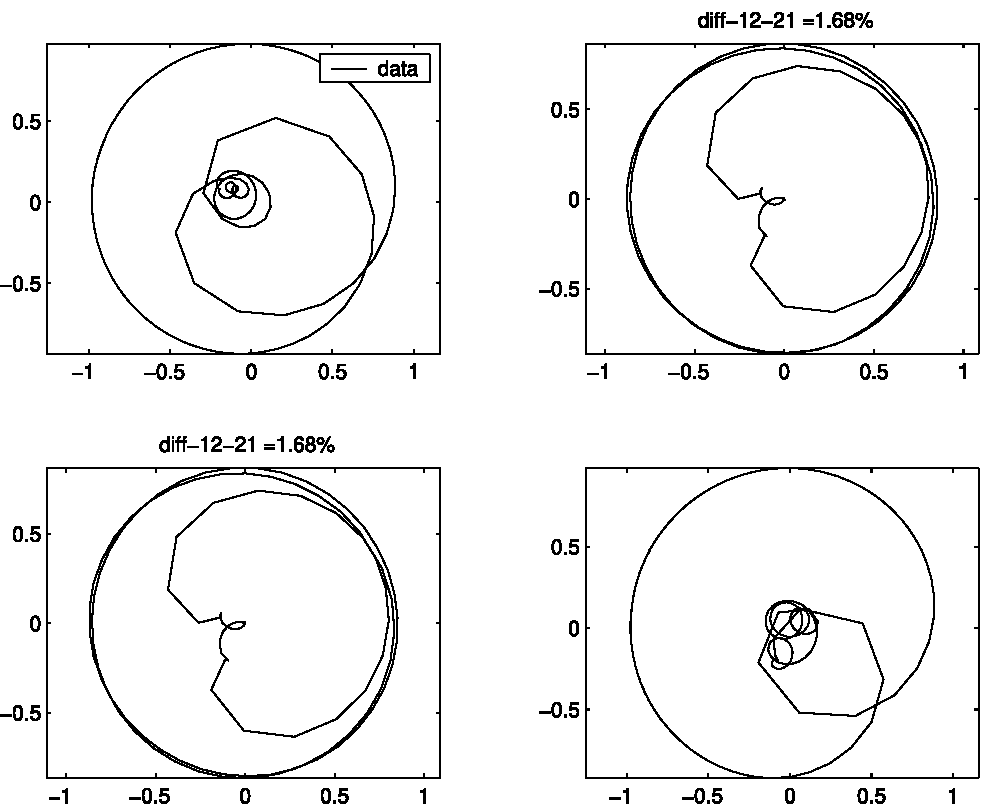
\includegraphics[width=0.8\linewidth]{Spbbrut.pdf}
\end{center}
\caption{Diagramme de Nyquist des donn\'ees}
\label{nyqSpb}
\end{figure}
\begin{figure}
\begin{center}
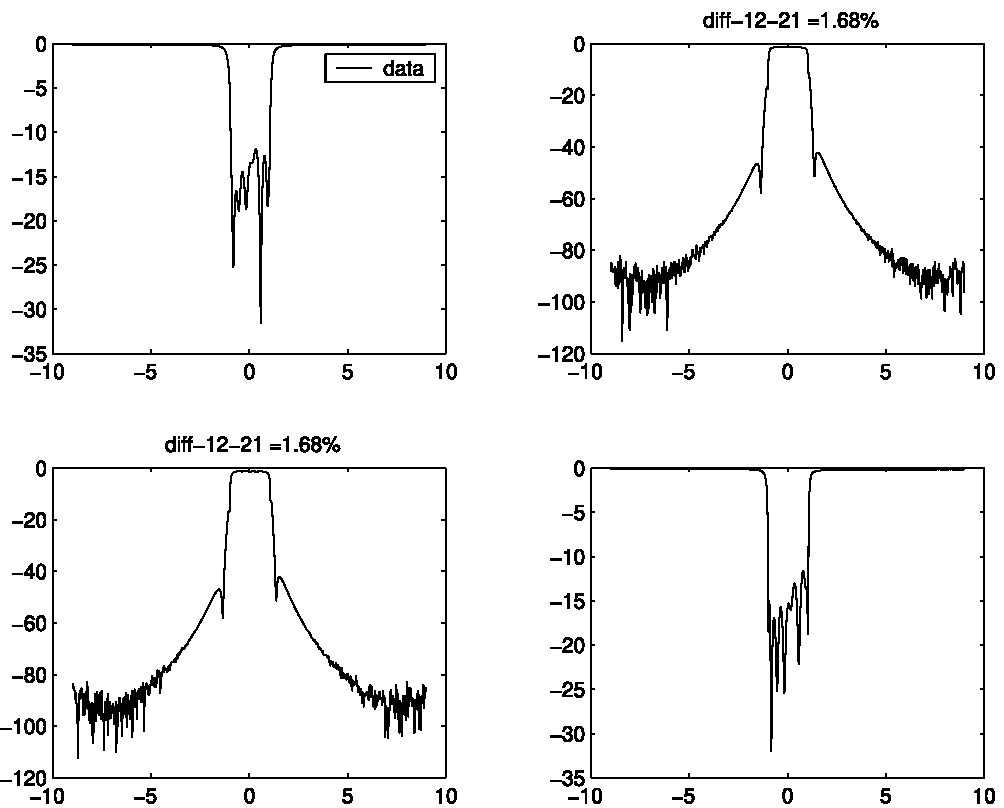
\includegraphics[width=0.8\linewidth]{Spbbode.pdf}  
\end{center}
\caption{Diagramme de Bode des donn\'ees}
\label{bodeSpb}
\end{figure}

  
\begin{figure}
\begin{center}
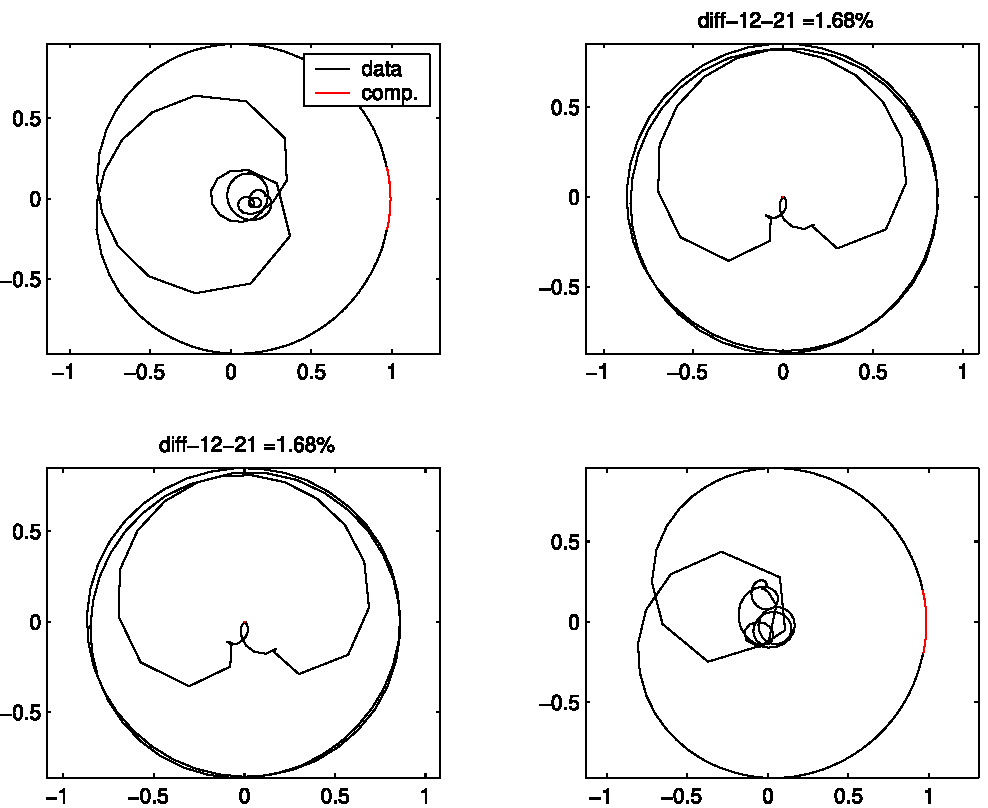
\includegraphics[width=0.8\linewidth]{Spbc.pdf}
\end{center}
\caption{Compl\'etion et donn\'ees}
\label{Spbc:fig}
\end{figure}
 
\begin{figure}
\begin{center}
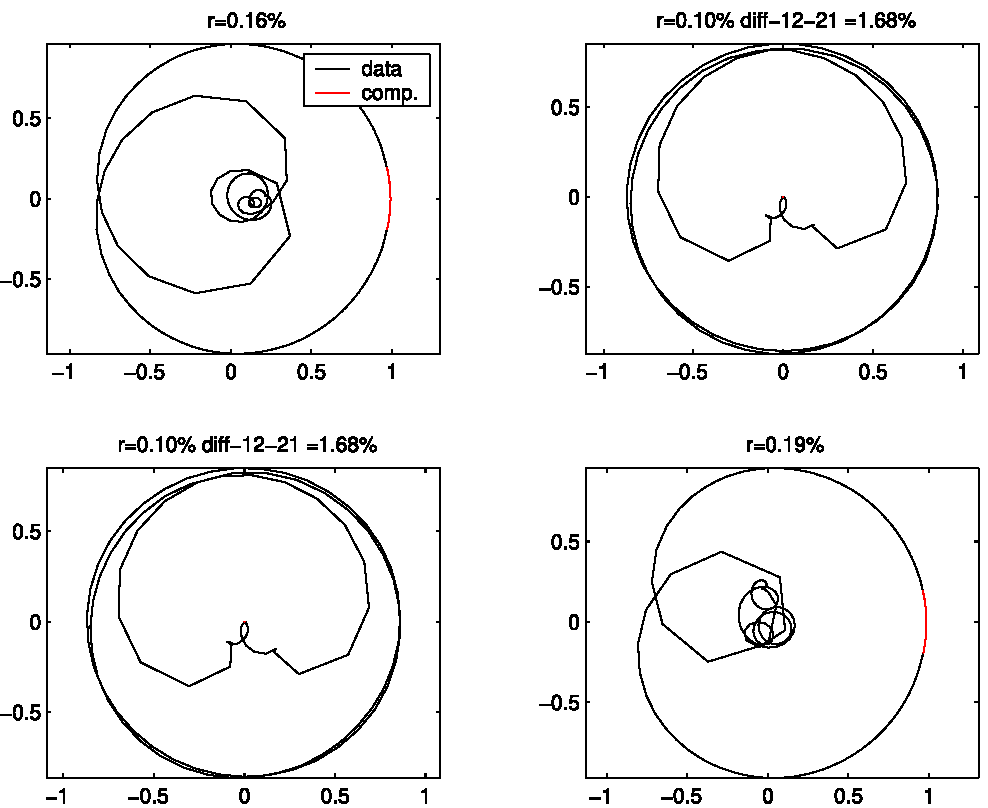
\includegraphics[width=0.8\linewidth]{Spbcfou.pdf}
\end{center}
\caption{Compl\'etion et donn\'ees apr\`es calcul coeff. Fourier}
\label{Spbcfou:fig}
\end{figure}

\begin{figure}
\begin{center}
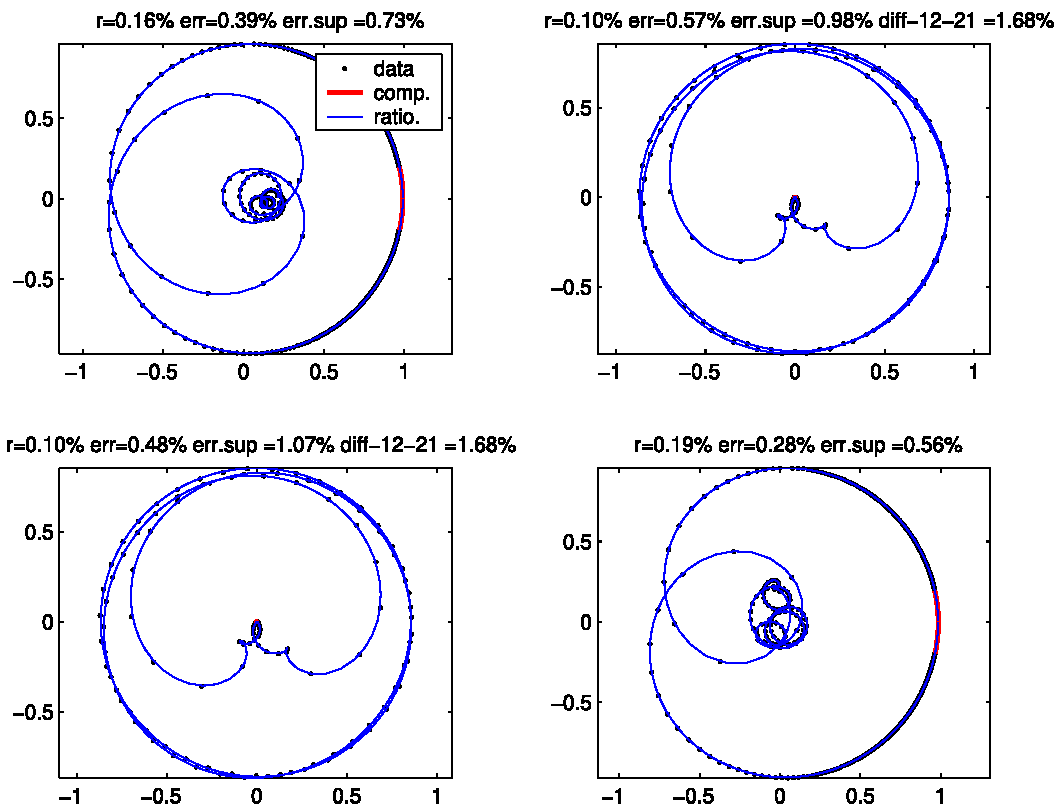
\includegraphics[width=0.8\linewidth]{Spbr.pdf}
\end{center}
\caption{Compl\'etion, donn\'ees et approximation rationnelle}
\label{Spbr:fig}
\end{figure}
        
   

\end{document}



